
\section{Experiments}
\label{sec:expts}
All code for the experiments is written in Python.
%
We use Matplotlib for plotting~\cite{hunter2007matplotlib} , scikit-learn for
machine-learning pipelines~\cite{pedregosa2011scikit}, MNE for MEG
processing~\cite{gramfort2013meg}, Nilearn for fMRI processing and for its CanICA implementation~\cite{abraham2014machine}, Brainiak~\cite{kumar2020brainiak} for its SRM implementation. 
%
In the following, the noise parameter in MultiviewICA is always fixed to $\sigma =1$.
%
We use the function $f(\cdot)= \log\cosh(\cdot)$, giving the non-linearity $f'(\cdot) = \tanh(\cdot)$.
%
We use the Infomax cost function~\cite{bell1995information} with the same non-linearity to perform standard ICA, with the Picard algorithm~\cite{ablin2018faster} for fast and robust minimization of the cost function. Picard is applied with the default hyper-parameters.
%
The code for MultiViewICA is available online at \url{https://github.com/hugorichard/multiviewica}.
%

We compare the following methods to obtain $k$ components:
%
\emph{GroupPCA} is PCA on spatially concatenated data. It corresponds to a transposed version of \cite{smith2014group}.
%
\emph{PermICA} is described in the previous section.
%
\emph{SRM} is  the algorithm of~\cite{chen2015reduced}.
%
\emph{GroupICA} is ICA applied after GroupPCA.
%
\emph{PCA+GroupICA} corresponds to GroupICA applied on subject data that have been first individually reduced by PCA with $k$ components. 
%
These two approaches correspond to transposed versions of~\cite{calhoun2001fmri}, and are similar to \cite{eichele2011eegift}.
\emph{CanICA} corresponds to PCA+GroupICA where the merging is done using multi set CCA rather than PCA. The dimension reduction in MultiView ICA and PermICA is performed with SRM in fMRI experiments and subject-specific PCA in MEG experiments. Initialization is discussed in appendix~\ref{sec:app_init}. A summary of our quantitative results on real data is available in appendix~\ref{sec:app_real_data}.

\begin{wrapfigure}{l}{0.4\textwidth}
\label{fig:synth}
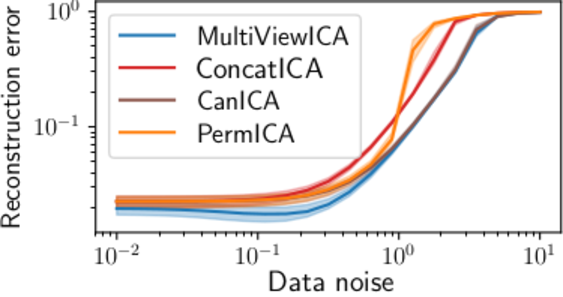
\includegraphics[width=0.38\textwidth]{figures/mvica/distance_expe.pdf}
\captionof{figure}{\textbf{Synthetic experiment}: reconstruction error of the algorithms on data following model~\eqref{eq:ica_model}.}
\end{wrapfigure}

\textbf{Synthetic experiment}
We validate our method on synthetic data generated according to the model in equation~\eqref{eq:ica_model}.
%
The sources are generated i.i.d. from a Laplace density $d(x)=\frac12\exp(-|x|)$.
%
The mixing matrices $A^1,\cdots, A^m$ are generated with i.i.d. entries following a normal law.
Each compared algorithm returns a sequence of estimated unmixing matrices $W^1, \dots, W^m$.
%
The performance of an algorithm is measured by the reconstruction error between the estimated sources and the true sources.
%$\frac1M\sum_{i=1}^Md(W^iA^i)$, where $d(P)=\sum_{i=1}^n \left(\sum_{j=1}^n\frac{|p_{ij}|}{\max_{k} |p_{ik}|} - 1\right) + \sum_{j=1}^n \left(\sum_{i=1}^n\frac{|p_{ij}|}{\max_{k} |p_{kj}|} - 1\right)$.
%
%This quantity cancels if and only if $P$ is a scale and permutation matrix.
%
We use $m=10$ datasets, $k=15$ sources and $n=1000$ samples. Each experiment is repeated with $100$ random seeds.
%
We vary the noise level in the data generation from $10^{-2}$ to $10$.

Multiview ICA has uniformly better performance than the other algorithms, which illustrates the strength of maximum-likelihood based methods. In accordance with results of section~\ref{sec:mvica}, it is able to separate the sources even with misspecified noise parameter and source density.
%
%\subsection{fMRI experiments}
%\label{sec:experiments}

\textbf{fMRI data and preprocessing} 
We evaluate the performance of our approach on four different fMRI datasets.
%
The \emph{sherlock} dataset~\cite{chen2017shared} contains recordings of 16 subjects watching an episode of the BBC TV show "Sherlock" (50 mins).
%
The \emph{forrest} dataset~\cite{hanke2014high} was collected while 19 subjects were listening to an auditory version of the film "Forrest Gump" (110 mins).
%
The \emph{clips} dataset~\cite{ibc} was collected while 12 participants were exposed to short video clips (130 mins).
%
The \emph{raiders} dataset~\cite{ibc} was collected while 11 participants were watching the movie "Raiders of the Lost Ark" (110 mins).
%
The \emph{raiders-full} dataset~\cite{ibc} is an extension of the \emph{raiders} dataset where the first two scenes of the movie are shown twice (130 mins).
%
Like \cite{zhang2016searchlight}, we used full brain data. The rest of the preprocessing is identical to \cite{chen2017shared}. See \ref{preprocessing} for a detailed description of the datasets and preprocessing steps. Unless stated otherwise we use spatially unsmoothed data, except for the \emph{sherlock} dataset, for which the available data are already preprocessed with a 6\,mm spatial smoothing. All datasets are built from successive acquisitions called \emph{runs} that typically last 10 minutes each.
%
We define the chance level as the performance of an algorithm that computes unmixing matrices and projections to lower dimensional space by sampling random numbers from a standard normal distribution. 
%

\textbf{Reconstructing the BOLD signal of missing subjects}
We want to show that once unmixing matrices have been learned, they can be
used to predict
evoked responses across subjects, which can be useful to perform transfer learning~\cite{zhang2018transfer}.
%
We split the data into three groups. First, we randomly choose $80\%$ of all runs from all subjects to form the training set.
%
Then, we randomly choose $80\%$ of subjects and take the remaining $20\%$  runs as testing set.
%
The left-out runs  of the remaining $20\%$ subjects form the validation set.
%
The compared algorithms are run on the training set and evaluated using the testing and validation sets.
%
After an algorithm is run on training data, it defines for each subject a \emph{forward operator} that maps individual data to the source space and a \emph{backward operator} that maps the source space to individual data. For instance in ICA the forward operator is the product of the dimensionality reduction projection and unmixing matrix.
%
We estimate the shared responses on the testing set by applying the forward operators on the testing data and averaging. Finally, we reconstruct the individual data from subjects in the validation set by applying the backward operators to the shared responses. We measure the difference between the true signal and the reconstructed one using voxel-wise $R^2$ score. The $R^2$ score between two series $\xb \in \bbR^n$ and $\yb \in \bbR^n$ is defined as
$R^2(\xb, \yb) = 1 - \frac1{n\Var(\yb)}\sum_{t=1}^n (x_t - y_t)^2$, where $\Var(\yb) = \frac1n\sum_{t=1}^n (y_t - \frac1n \sum_{t'=1}^n y_{t'})^2$ is the empirical variance of $\yb$.
%
The $R^2$ score is always smaller than $1$, and equals $1$ when $\xb= \yb$.
The experiment is repeated 25 times with random splits to obtain error bars.


In this experiment we apply a 6\,mm spatial smoothing to all datasets. The $R^2$ score per
voxel depends heavily on which voxel is considered. For example voxels in the
visual cortex are better reconstructed in the \emph{sherlock} dataset than in
the \emph{forrest} dataset (see Figure~\ref{fig:brainmaps} in appendix~\ref{brainmaps}). In Figure~\ref{fig:reconstruction}
(top) we plot the mean $R^2$ score inside a region of interest (ROI) in order to leave out regions where there is no useful information.
%
ROIs are chosen based on the performance of GroupICA (more
details in appendix~\ref{brainmaps}).
%
MultiView ICA has similar or better performance than the other methods on all datasets.
%
This demonstrates its ability to capture inter-subject variability, making it a candidate of choice to handle missing data or perform transfer learning.

\begin{figure}
  \centering
  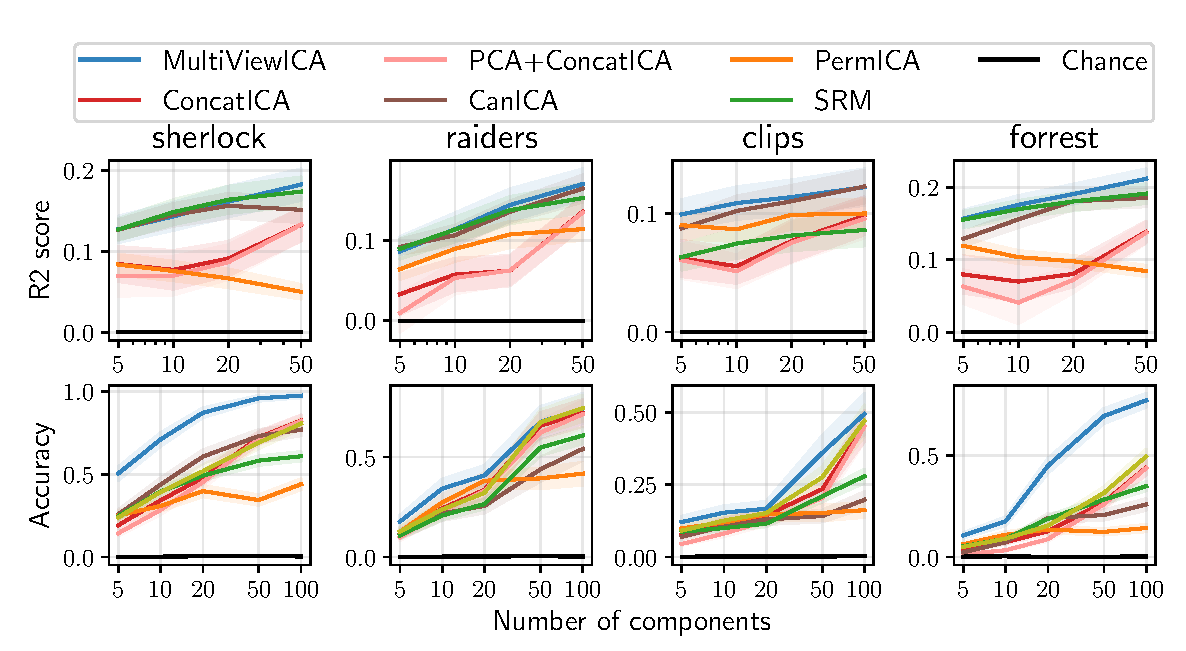
\includegraphics[width=0.9\textwidth]{figures/mvica/timesegment_matching_reconstruction.pdf}
  \caption{\emph{Top:} \textbf{Reconstructing the BOLD signal of
      missing subjects}. Mean $R^2$ score between reconstructed data and true
    data (higher is better). \emph{Bottom:} \textbf{Between subjects time-segment matching}. Mean
    classification accuracy. Error bars represent a 95 \% confidence interval over cross validation splits.}
  \label{fig:reconstruction}
  \label{fig:timesegment}
\end{figure}


\textbf{Between subjects time-segment matching} 
We reproduce the time-segment matching experiment of
\cite{chen2015reduced}. 
We split the runs into a train and test set. After fitting the model on the training set, we apply the forward operator of each subject on the test set yielding individual sources matrices. We estimate the shared responses by averaging the individual sources of each subjects but one.  We select a target time-segment (9 consecutive timeframes) in the shared responses and try to localize the corresponding time segment in the sources of the left-out subject using a maximum-correlation classifier.
This is a standard evaluation of SRM-like methods also used in  \cite{chen2015reduced}, \cite{guntupalli2018computational}, \cite{Nastase741975} or
\cite{zhang2016searchlight}.
%
The time-segment is said to be
correctly classified if the correlation between the sample and target
time-segment is higher than with any other time-segment (partially overlapping time windows are excluded).
%
We use 5-Fold cross-validation across runs: the training set contains 80\% of the runs and the test set 20\%, and repeat the experiment using all possible choices for left-out subjects. 
%
The mean accuracy is reported in Figure~\ref{fig:timesegment} (bottom). 
%
MultiView ICA yields a consistent and substantial improvement in accuracy compared to other methods on the four datasets. We see a marked improvement on the datasets sherlock and forrest. A possible explanation lies in the preprocessing pipeline. Sherlock data undergo a 6~mm spatial smoothing and Forrest data are acquired at a higher resolution (7T vs 3T for other data). This affects the signal to noise ratio.
%
In appendix~\ref{sec:app_sigma_impact}, we compute the accuracy of MultiviewICA on the sherlock dataset with 10 components when the noise parameter varies. MultiviewICA performs consistently well for a wide range of noise parameter values, and only breaks at very high values. It supports the theoretical claim of Prop~\ref{prop:robust} that the noise parameter is of little importance.

In appendix~\ref{app_spatialmaps}, we present a variation of this experiment.  We measure the ability of each algorithm to extract meaningful shared sources that correlate more when they correspond to the same stimulus than when they correspond to distinct stimuli and show the improved performance of MultiView ICA. 
%
In appendix~\ref{sec:spatial_maps}, we plot the average forward operator across subjects of MultiView ICA and GroupICA with 5 components on the forrest, sherlock, raiders and clips datasets.

%\subsection{MEG experiments}
\textbf{Phantom MEG data}
We demonstrate the usefulness of our approach on MEG data.
%
The first experiment uses data collected with a realistic head phantom, which is a plastic device mimicking real electrical brain sources.
%
Eight current dipoles positioned at different locations can be switched on or off.
%
We view each dipole as a subject and therefore have $m=8$.
%
We only consider the 102 magnetometers.
%
An epoch corresponds to 3\,s of MEG signals where a dipole is switched on for 0.4\,s with an oscillation at 20\,Hz and a peak-to-peak amplitude of 200\,nAm.
%
This yields a matrix of size $p\times n$ where $p=102$ is the number of sensors, and $n$ is the number of time samples.
%
We have access to $100$ epochs per dipole.
%
For each dipole, we chose $N_e=2, \dots, 16$ epochs at random among our set of 100 epochs and concatenate them in the temporal dimension.
%
We then apply algorithms on these data to extract $k=20$ shared sources.
%
As we know the true source (the timecourse of the dipole), we can compute the reconstruction error of each source as the squared norm of the difference between the estimated source and the true source, after normalization to unit variance and fixing the sign.
%
We only retain the source of minimal error.
%
We also estimate for each forward operator the localization of the source by performing dipole fitting using its column corresponding to the source of minimal error.
%
We then compute the distance of the estimated dipole to the true dipole.
%
These metrics are reported in figure~\ref{fig:meg} when the number of epochs considered $N_e$ varies.
%
We also compare our method to the Bayesian Canonical Correlation Analysis (BCorrCA) of~\cite{kamronn2015multiview}.
%
On this task, BCorrCA is outperformed by ICA methods.
%
MultiView ICA requires fewer epochs to correctly reconstruct and localize the true source.
%

\textbf{Experiment on Cam-CAN dataset}
Finally, we apply MultiView ICA on the Cam-CAN dataset~\cite{taylor2017cambridge}. We use the magnetometer data from the MEG of $200$ subjects.
%
Each subject is repeatedly presented an audio-visual stimulus. 
%
The MEG signal corresponding to these trials are then time-averaged to isolate the evoked response, yielding individual data.
%
The MultiView ICA algorithm is then applied to extract $20$ shared sources.
%
$9$ sources were found to correspond to noise by visual inspection, and the $11$ remaining are displayed in figure~\ref{fig:meg}.
%
We observe that MultiView ICA recovers a very clean sequence of evoked potentials with sharp peaks
for early components and slower responses for late components.
%
In order to visualize their localization, we perform source localization for each subject by solving the inverse problem using sLORETA~\cite{pascual2002standardized}, providing a source estimate for each source.
%
Then, we register each source estimate to a common reference brain.
%
Finally, the source estimates are averaged, and thresholded maps are displayed in figure~\ref{fig:meg}.
%
Individual maps corresponding to each source are displayed in appendix~\ref{sec:app_montages}.
The figure highlights both early auditory and visual cortices, also suggesting a propagation
of the activity towards the ventral regions and higher level visual areas.

\begin{figure}
    \centering

          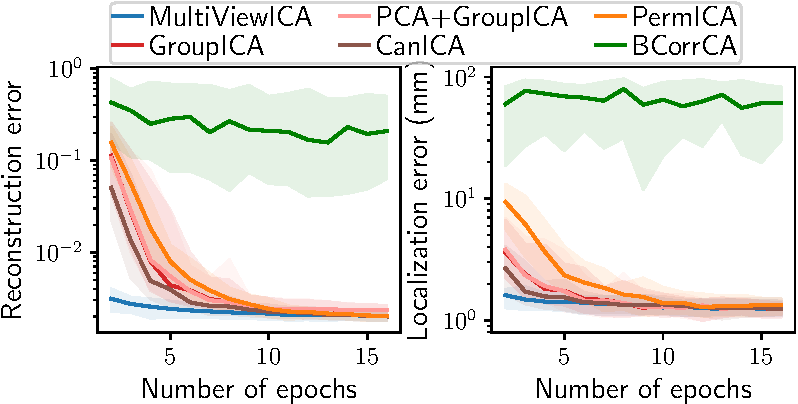
\includegraphics[width=0.4\linewidth]{figures/mvica/phantom_new.pdf}
          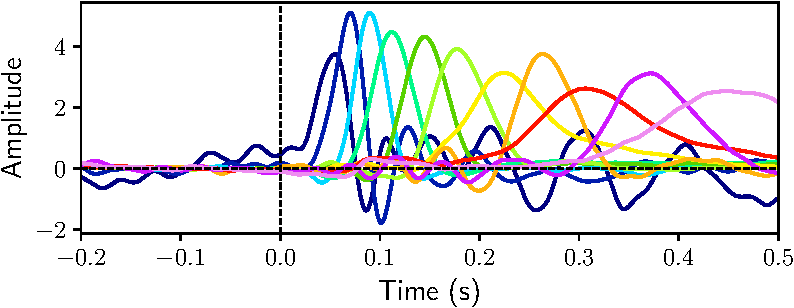
\includegraphics[width=0.4\textwidth]{figures/mvica/camcan_sources.pdf}
          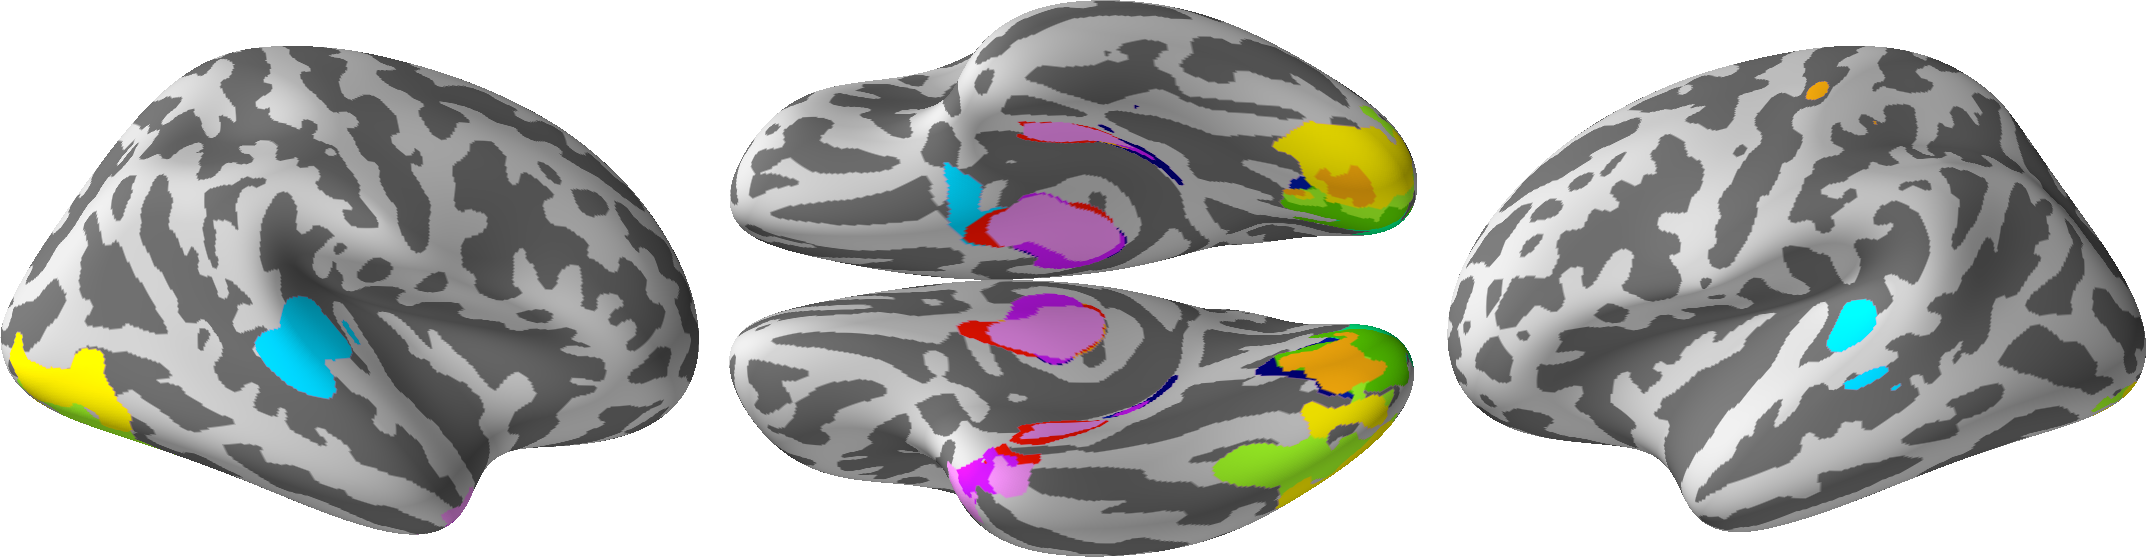
\includegraphics[width=0.4\textwidth]{figures/mvica/montage_all.png}
    \caption{\emph{Left:} \textbf{Experiment on MEG Phantom data}. Reconstruction error is the norm of the difference between the estimated and true source. Localization error is the distance between the estimated and true dipole. \emph{Right:} \textbf{Experiment on 200 subjects from the CAM-can dataset} \emph{Top:} Time course of $11$ shared sources (one color per source). We recover clean evoked potentials. \emph{Bottom:} Associated brain maps, obtained by averaging source estimates registered to a common reference.}
    \label{fig:meg}
\end{figure}

\vspace{-11pt}
%
%
% \section{Conclusion}
% \label{sec:disc}
% \input{sec/conclusion}
%
%
%\section{Conclusions}
%\label{sec:conclusions}
%We propose a new method for modeling shared responses in neuroimaging studies. The method is identifiable and, overall, it rocks.
%
%
% \section*{References}
% \section*{Broader Impact}
% We develop a novel unsupervised learning method for Independent Component Analysis of a group of subjects sharing commmon sources.
% %
% Our method is not limited to a particular type of data, and could hence be employed in observational sciences where ICA is relevant: neurosciences, genomics, astrophysics, finance or computer vision for instance.
% %
% ICA is widely used in these fields as a tool among data processing pipelines, and therefore inherits from all the ethical questions of the fields above.
% %
% In particular, data collection bias will result in biased outputs.
% %
% Our algorithm is based on individual linear transforms and therefore decisions based on its application are easier to interpret than more complex models such as deep learning methods: in most applications, the set of parameters has a natural interpretation. For instance in EEG, MEG and fMRI processing, the coefficients of the linear operator can be interpreted as topographic brain maps. 


% \section*{Acknowledgement and funding disclosure}

% This work was supported in part by the French government under management of Agence Nationale de la Recherche as part of the “Investissements d'avenir” program, references ANR19-P3IA-0001 (PRAIRIE 3IA Institute) and ANR17-CONV-0003 (DataIA Institute). It has also received funding from the European Union’s Horizon 2020 Framework Programme for Research and Innovation under the Specific Grant Agreement No. 945539 (Human Brain Project SGA3), the KARAIB AI chair (ANR-20-CHIA-0025-01) and the European Research Council grant ERC-SLAB-StG-676943. L.G. was hosted for part of this project by the Parietal team at Inria, Saclay, while on an ELLIS exchange. A.H. was additionally supported by CIFAR as a Fellow.
